\chapter{\MakeUppercase{Механическая конструкция}}
\section{Проектирование ног} \label{sec:leg_design}
Основная, и самая сложная с точки зрения механики часть шагающего робота, это конечности. Как и корпус, ноги проектировались в виде трёхмерных, твердотельных чертежей. Для уменьшения количества уникальных деталей конструкция всех четырех ног была унифицирована. Таким образом снижена сложность и затратность в производстве деталей. 

\begin{figure}[h]
    \centering
    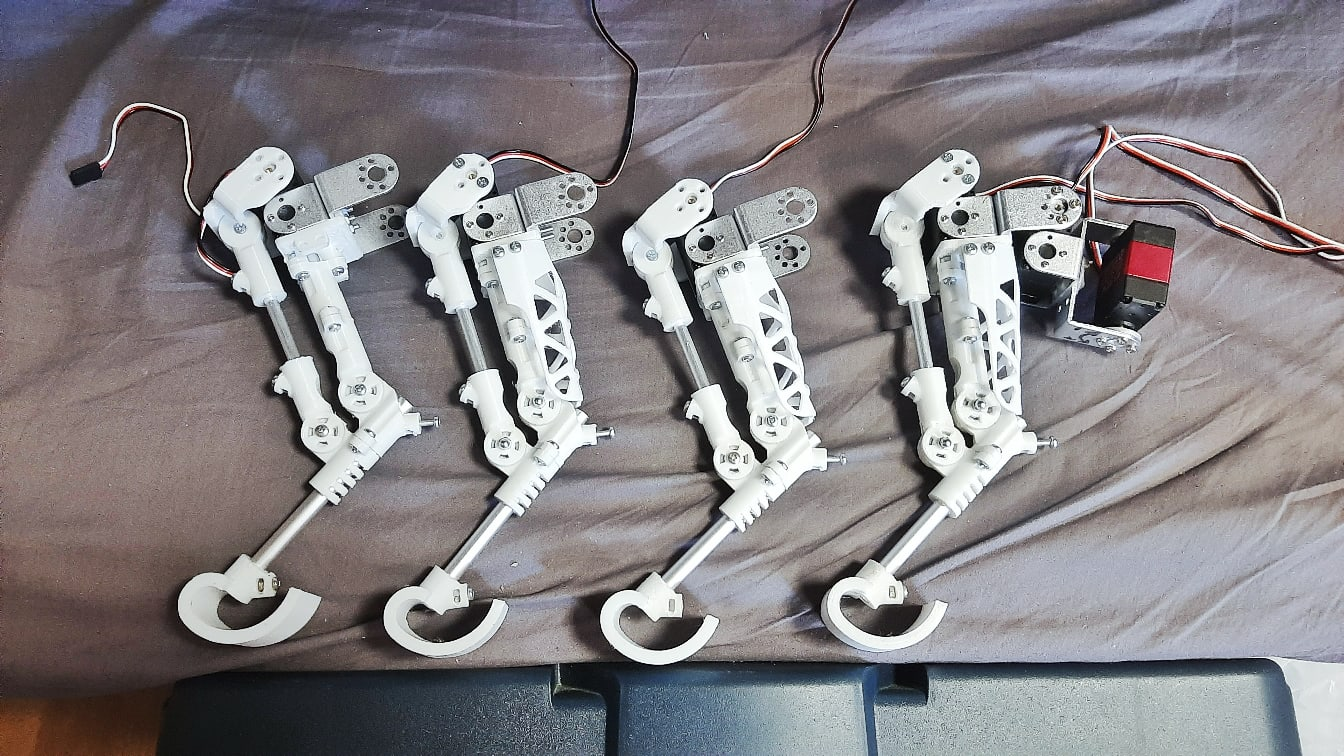
\includegraphics[width=\textwidth]{chapter_mechanics_construction/figure11.jpg}
    \caption{Конструкции всех четырех ног унифицированы}
    \label{}
\end{figure}

Сложные по форме детали изготовлены из пластика на 3D-принтере, в конструкции также присутствуют металлические стержни, стандартные металлические кронштейны, крепежные элементы (винты, гайки).

Перед проектированием были выдвинуты функциональные требования к конечностям. Они должны быть как можно менее габаритными, для сохранности редукторов сервоприводов и для увеличения скорости движения нужно максимально уменьшить момент инерции конечности. Основной способ достижения этой цели -- уменьшение веса всех деталей. Поэтому крепежные и элементы корпуса, были изготовлены из пластика, там где это было возможно. Были использованы полые цилиндрические аллюминиевые трубки в качестве стержней, обеспечивающих жесткость.

\begin{figure}[h]
    \centering
    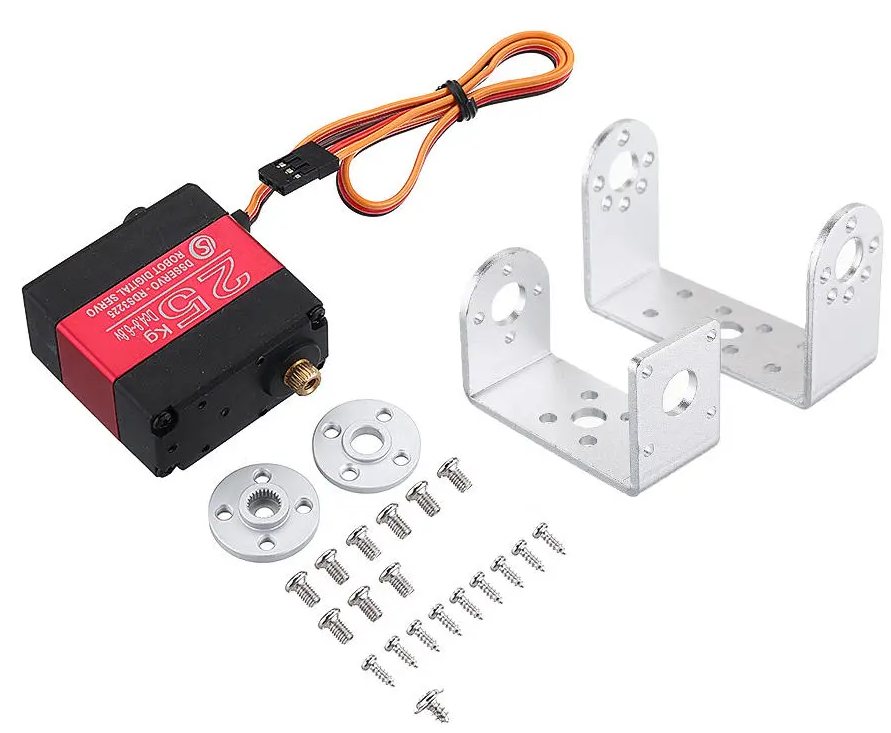
\includegraphics[scale=0.45]{chapter_mechanics_construction/figure6.png}
    \caption{Сервоприводы \textit{DSSERVO RDS3225}, использованные в прототипе робота}
    \label{}
\end{figure}

Есть еще один, не менее эффективный способ снизить момент инерции ног, не уменьшая общего веса конечностей -- концентрация основной массы как можно выше \cite{Seok2012}, ближе к месту крепления ноги к корпусу. Поэтому сервоприводы, как одни из самых тяжелых элементов конструкции, были перенесены максимально близко к корпусу и максимально далеко от пола.

\begin{figure}[h]
    \centering
    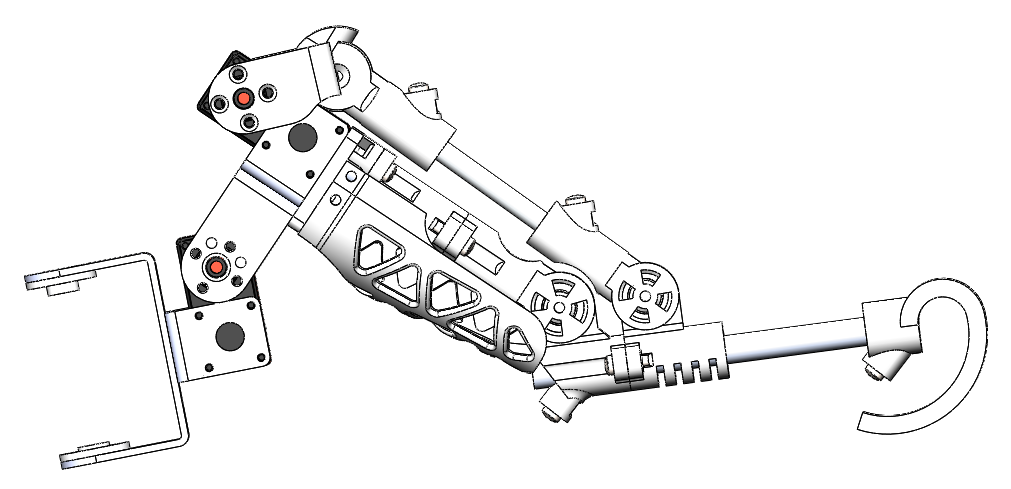
\includegraphics[scale=0.7]{chapter_mechanics_construction/figure7.png}
    \caption{Твердотельный чертеж конечности робота. Можно заметить что двигатели размещены у основания конечности.}
    \label{}
\end{figure}

В связи с этим в конструкции возник механический четырехзвенник, позволяющий для вращения последнего звена установить сервопривод не непосредственно в шарнир, а передать вращение вала издалека. Четырехзвенник усложнил кинематическую схему ноги, его расчет рассмотрен далее в пункте \ref{sec:pre_direct_kin}, однако такая конструкция не только хорошо повлияла на механические характеристики ноги, но и на эстетические тоже. Крутящий момент передается при помощи четырехзвенной передачи и двигатель, который имеет неоптимальные габариты, не пришлось размещать в последнем узле ноги, что позволило сделать конечность максимально компактной.

\begin{figure}[h]
    \centering
    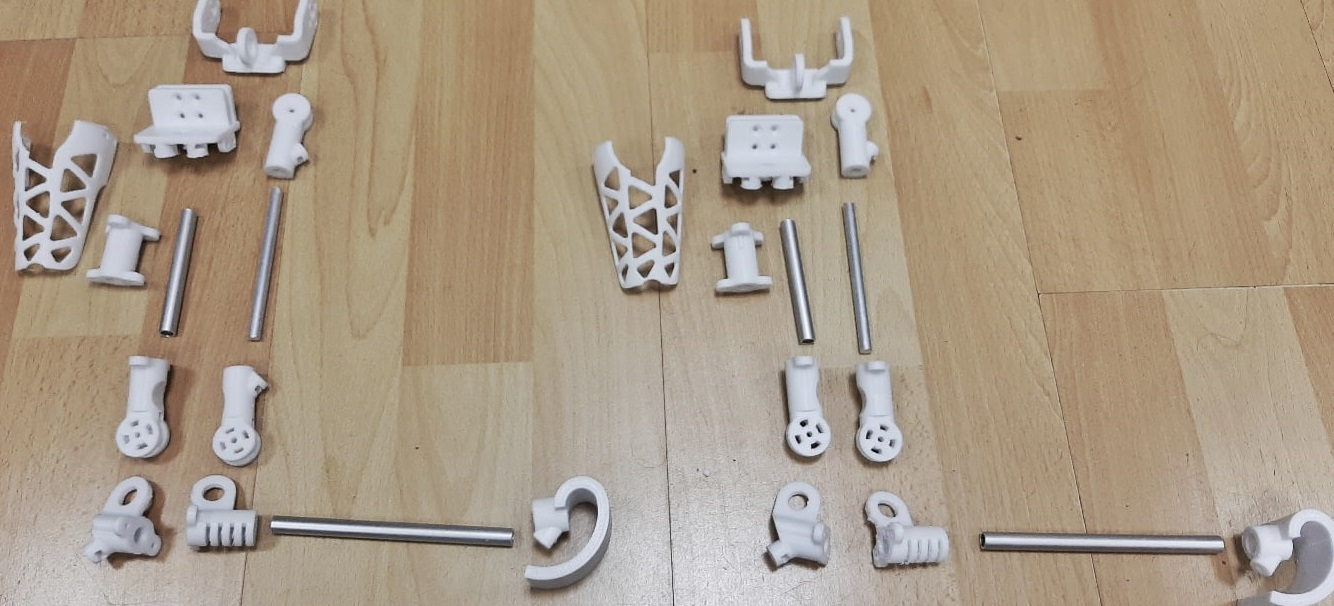
\includegraphics[width=\textwidth]{chapter_mechanics_construction/figure14.jpg}
    \caption{Набор унифицированных деталей для изготовления конечностей.}
    \label{}
\end{figure}

\begin{figure}[h]
    \centering
    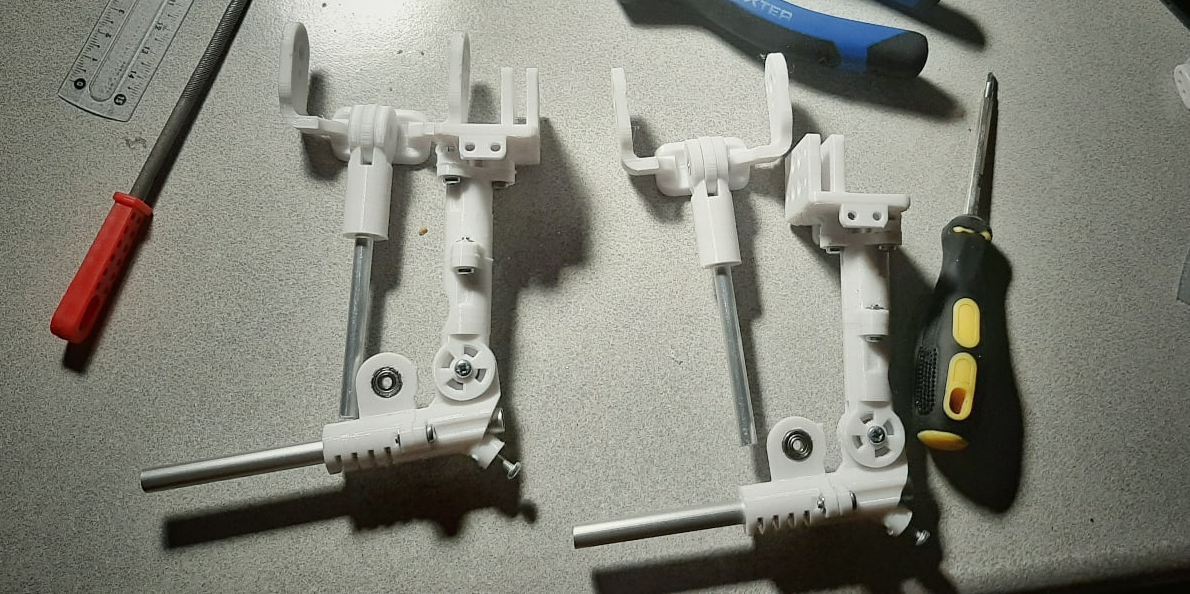
\includegraphics[width=\textwidth]{chapter_mechanics_construction/figure12.png}
    \caption{Процесс сборки конечностей. Используются полые аллюминиевые стержни и пластиковые детали.}
    \label{}
\end{figure}

В конструкции предусмотрена установка датчиков касания на стопы, в ходе развития проекта. Стопы можно будет заменить на более совершенные, а конструкция ноги позволит без проблем проложить провода внутри стержней, либо сокрытыми за стенками корпуса.
\begin{figure}[ht]
    \centering
    % левая картинка
    \begin{subfigure}[b]{0.45\textwidth}    
        \centering
        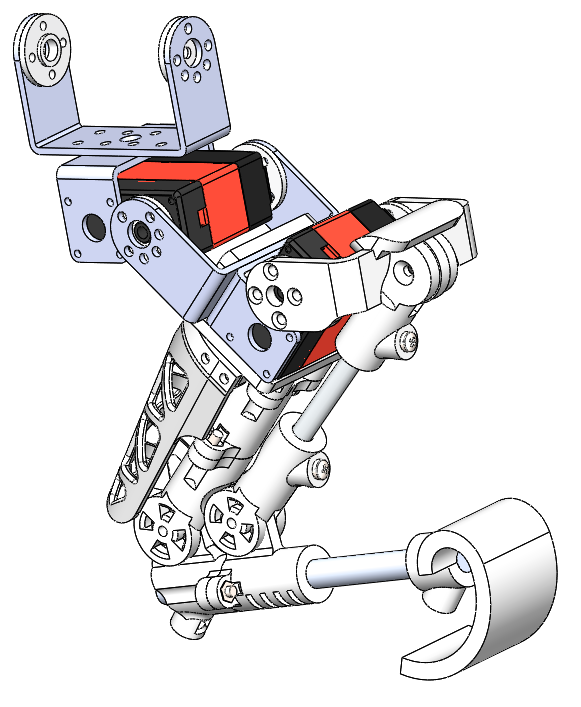
\includegraphics[scale=0.55]{chapter_mechanics_construction/figure15.png}
        \caption{Последнее звено согнуто}
    \end{subfigure}
    % правая картинка  
    \begin{subfigure}[b]{0.45\textwidth}
        \centering
        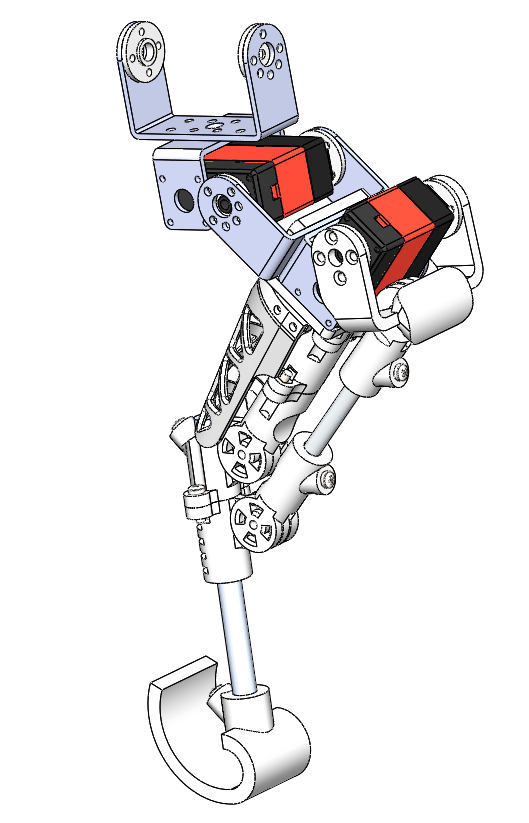
\includegraphics[scale=0.55]{chapter_mechanics_construction/figure16.png}
        \caption{Последнее звено разогнуто}
    \end{subfigure}
     
    \caption{Конечность в двух состояниях}
    \label{}
\end{figure}

Из-за специфики сервоприводов возникают проблемы во время сборки, которые замедляют процесс сборки и требуют наличия управляющей электроники. Дело в том что при установке в конструкцию ноги, сервопривод должен быть верно сконфигурирован, или проще говоря, быть заранее повернутым на известный далее управляющей программе угол поворота. Так называемый технический угол. Этим минусом обладают все сервоприводы такого типа. В других видах приводов конфигурировать углы поворота при сборке не нужно, но каждый раз при запуске нужно калибровать приводы, поворачивая их в нулевое, начальное положение. Такие приводы не были использованы в силу своей дороговизны и в силу того что наличие концевых выключателей в конструкции конечности сильно бы усложнило разработку. Для прототипа это излишне.

\section{Проектирование корпуса}
Требования к корпусу можно разделить на три составляющие: массовые, габаритные и эстетические. Снижать массу нужно для того чтобы разгрузить конечности робота, защитить редукторы электроприводов. Снижению массы способствует максимальный отказ от металлических деталей, а там где это невозможно (в силу требований по жесткости), нужно использовать эффективные сечения профилей, желательно из аллюминия.

В качестве каркаса, к которому крепятся ноги робота был выбран конструкционный аллюминиевый профиль, из-за его легкости, жесткости и простоты крепления новых деталей к профилю.
\begin{figure}[ht]
    \centering
    % левая картинка
    \begin{subfigure}[b]{0.45\textwidth}    
        \centering
        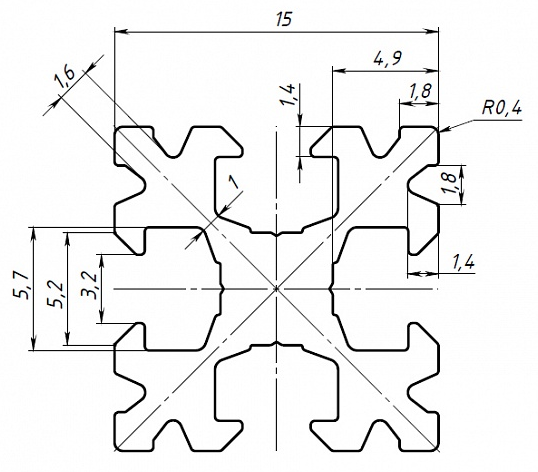
\includegraphics[scale=0.75]{chapter_mechanics_construction/figure8.png}
        \caption{Сечение профиля}
    \end{subfigure}
    % правая картинка  
    \begin{subfigure}[b]{0.45\textwidth}
        \centering
        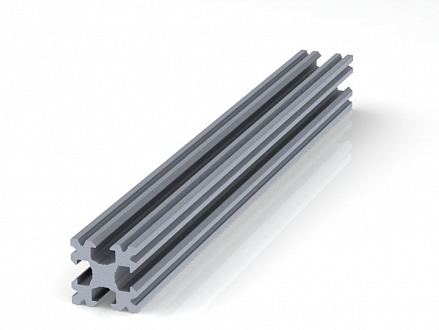
\includegraphics[scale=0.9]{chapter_mechanics_construction/figure9.png}
        \caption{Внешний вид профиля}
    \end{subfigure}
     
    \caption{Конструкционный аллюминиевый профиль}
    \label{}
\end{figure}

Объем корпусу придают тонкие цилиндрические аллюминиевые стержни и пластиковые детали в качестве передней и задней стенки. В узлах между металлическими профилями используются пластиковые крепежи. Такая конструкция позволяет использовать максимально много места внутри корпуса, что упрощает размещение электронных компонентов внутри.

\begin{figure}[h]
    \centering
    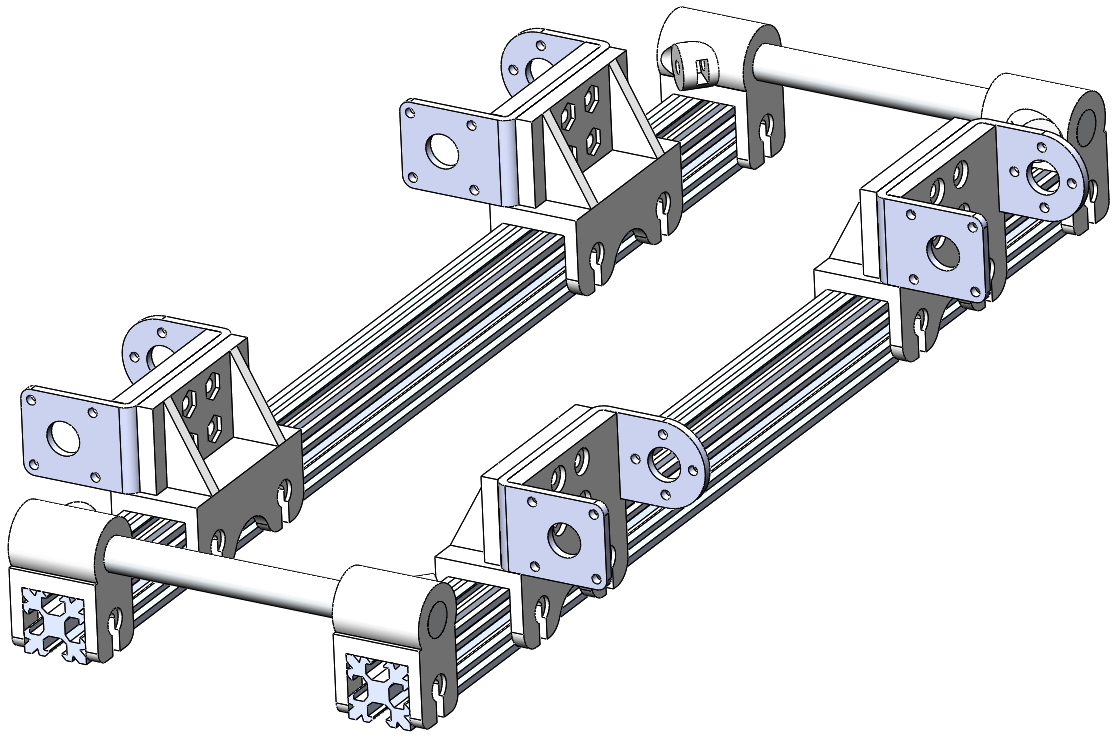
\includegraphics[scale=0.55]{chapter_mechanics_construction/figure10.png}
    \caption{Основной каркас корпуса}
    \label{}
\end{figure}

\newpage
Самой сложной задачей была компоновка всех компонентов внутри корпуса, так как нужно сохранить их <<доступность>> в любой момент времени для замены или диагностики. Таким образом повышается общая ремонтопригодность прототипа, а это сильно ускоряет работу с ним.

\begin{figure}[h]
    \centering
    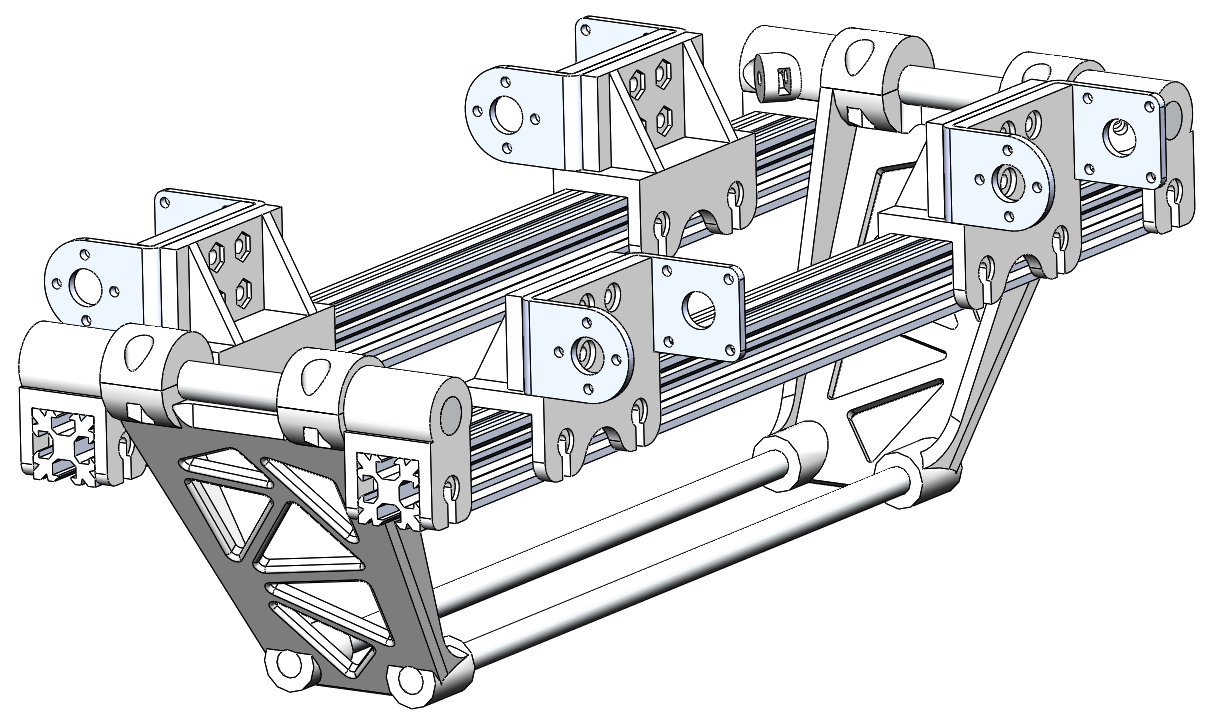
\includegraphics[scale=0.57]{chapter_mechanics_construction/figure13.png}
    \caption{Короб, скрепленный с корпусом}
    \label{}
\end{figure}

Чтобы максимально облегчить работу над монтажем электроники, был разработан электронный блок, целиком вынимающийся из корпусного короба. У такого решения есть как преимущества, так и недостатки. Важно что в таком состоянии сохраняется <<наглядность>> электронной схемы, легкий доступ воздуха к компонентам, исключающий факт перегрева и последующего выхода из строя по причине того что перегрев не был вовремя замечен.

\fixme ИЛЛЮСТРАЦИЯ ЭЛЕКТРОННОГО БЛОКА



\section{Подбор комплектующих}
\subsection{Силовая электроника}
Из силовой электроники в роботе присутствуют:
\begin{itemize}
    \item Сервоприводы
    \item \textit{DC-DC} преобразователи напряжения.
\end{itemize}

Исходя из ожидаемых моментов и скоростей был выбран заводской сервопривод \textit{DSSERVO RDS3225}.

Использовать паспортные данные двигателей для расчётов может быть рискованно, нужно измерить их реальный момент вращения. Для измерения крутящих моментов были разработаны стенды, принцип действия которых можно описать следующей схемой:

\begin{figure}[ht]
    \centering
    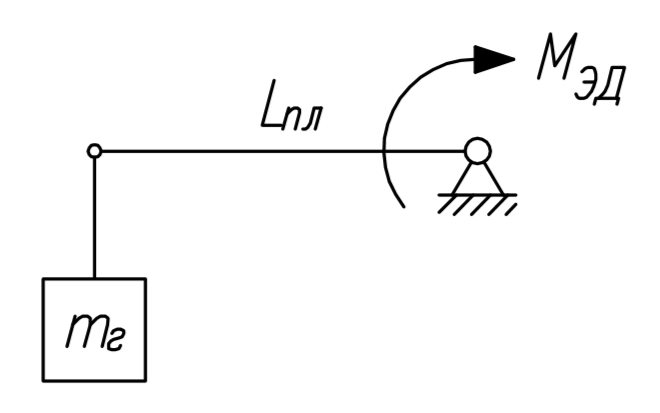
\includegraphics[scale=0.7]{chapter_legged_robots/kin3.png}
    \caption{Кинематика стенда для измерения крутящего момента}
\end{figure}

На изображении $ m_г $ - масса груза, которая нам известна, и которую мы можем менять. $ L_{пл} $ - длина плеча, также известная нам. Из приведенных величин можно легко найти экспериментально значение момента $ M_ {ЭД} $. После проверки сервопривода на стенде, оказалось что действительная величина крутящего момента соответствует паспортным данным в пределах погрешности измерений.

Преобразователи напряжения используются максимально компактные и простые в настройке. В основном используются испульсные преобразователи на базе микросхем \textit{LM-XXXX} и \textit{XL-XXXX}. Они хорошо взаимозаменяемы друг с другом. Для двух пар ног выбраны два преобразователя с максимальным током нагрузки $ 5 \: А $. Для питания логической части используется преобразователь с током нагрузки $ 3 \: А $.
\begin{figure}[ht]
    \centering
    % левая картинка
    \begin{subfigure}[b]{0.45\textwidth}    
        \centering
        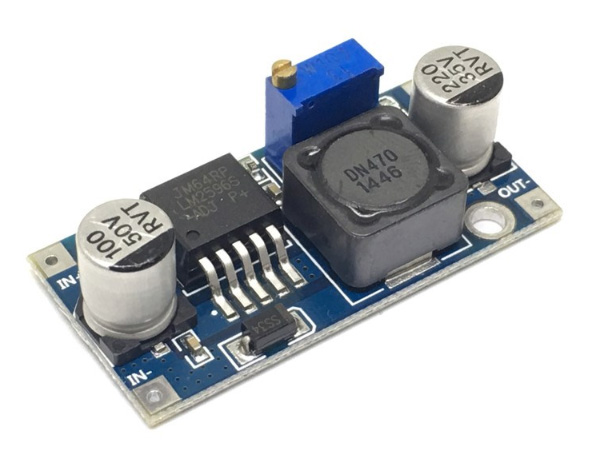
\includegraphics[scale=0.30]{chapter_mechanics_construction/figure4.jpg}
        \caption{Преобразователь на базе \textit{LM2596S}}
    \end{subfigure}
    % правая картинка  
    \begin{subfigure}[b]{0.45\textwidth}
        \centering
        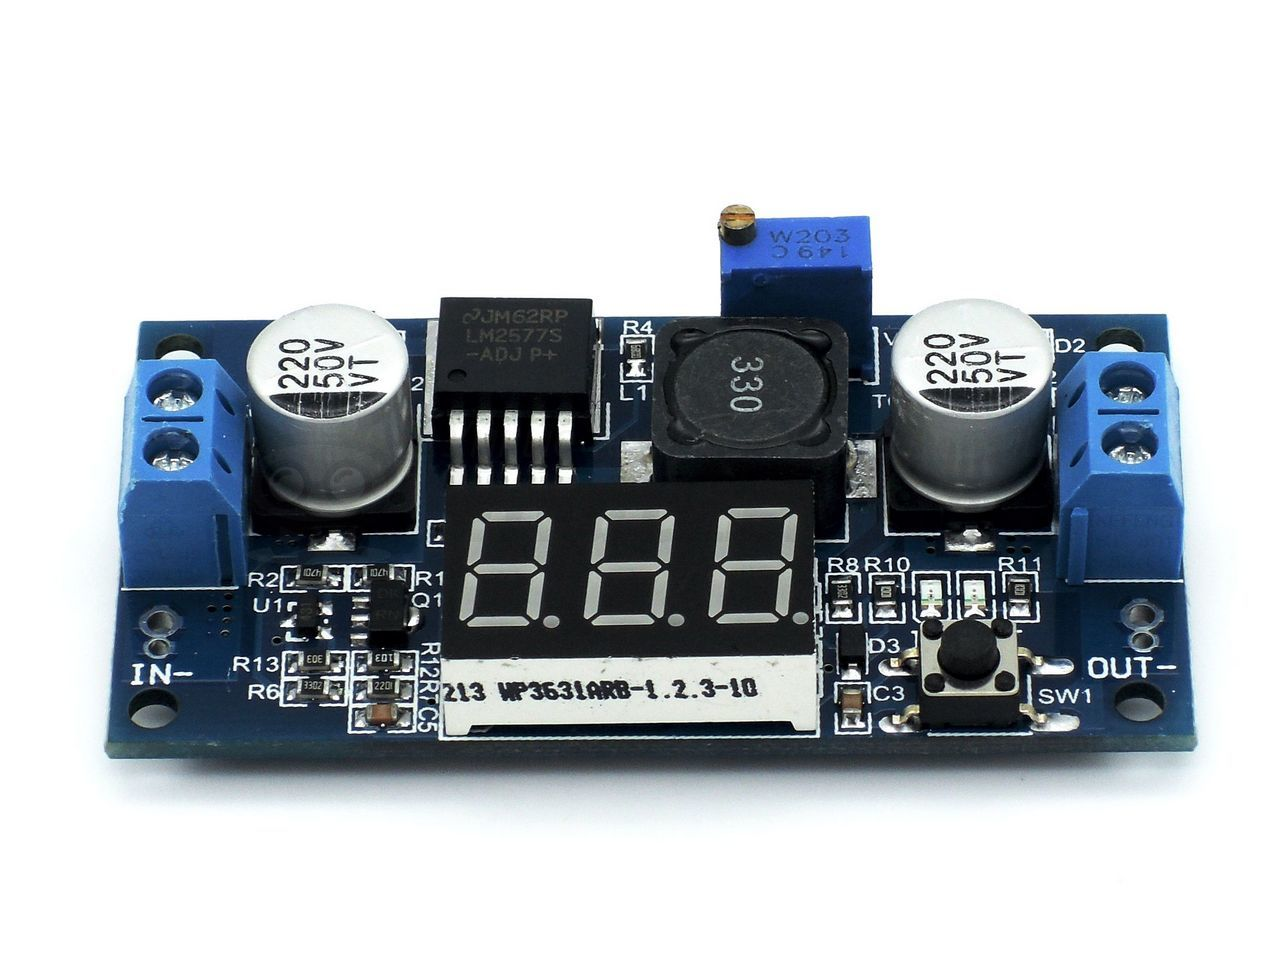
\includegraphics[scale=0.15]{chapter_mechanics_construction/figure5.jpg}
        \caption{Преобразователь на базе \textit{LM2577}}
    \end{subfigure}
     
    \caption{Некоторая силовая электроника в составе робота}
    \label{}
\end{figure}

\subsection{Логическая электроника}
В качестве управляющего микрокомпьютера выступает \textit{Raspberry Pi 3B+}. Этого достаточно для совершения множества матричных операций в секунду и для эффективной работы с высокоуровневыми абстракциями в коде.

\begin{figure}[ht]
    \centering
    % левая картинка
    \begin{subfigure}[b]{0.45\textwidth}    
        \centering
        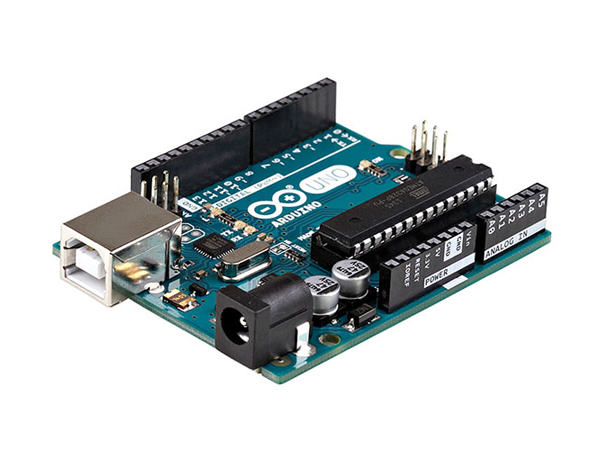
\includegraphics[scale=0.35]{chapter_mechanics_construction/figure3.jpg}
        \caption{\textit{Arduino Uno}}
    \end{subfigure}
    % правая картинка  
    \begin{subfigure}[b]{0.45\textwidth}
        \centering
        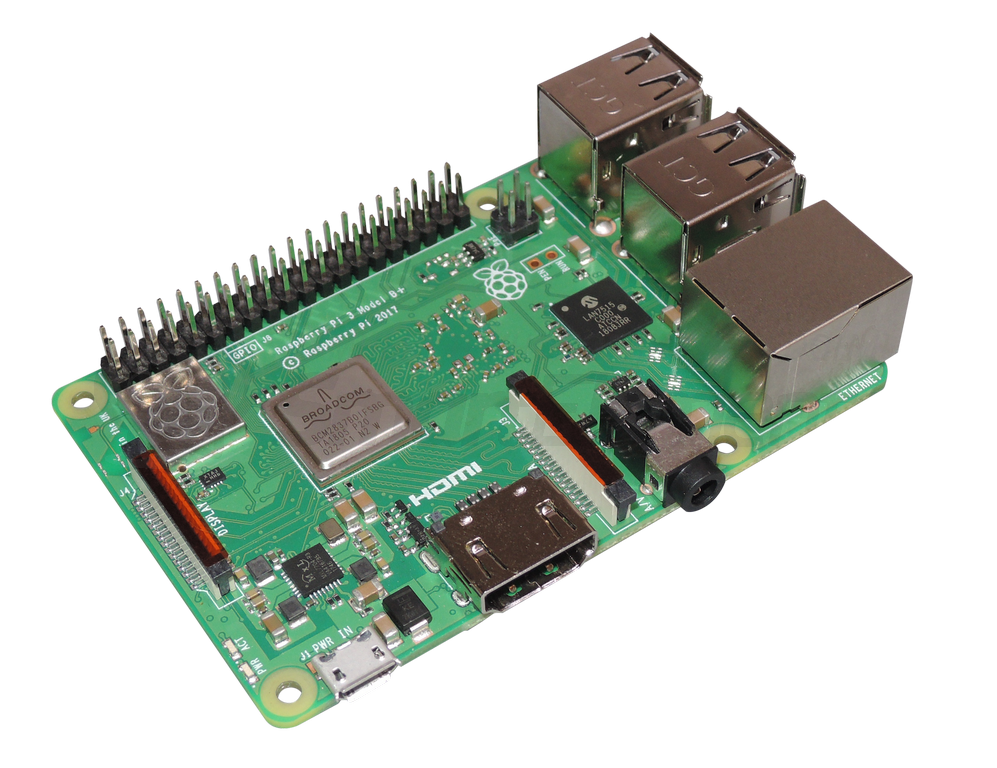
\includegraphics[scale=0.2]{chapter_mechanics_construction/figure3.png}
        \caption{\textit{Raspberry Pi 3B+}}
    \end{subfigure}
     
    \caption{Логическая электроника в составе робота}
    \label{fig:leg_model}
\end{figure}

\textit{Raspberry Pi} выступает исключительно как своеобразный модуль для высокоуровневых вычислений и не работает с <<железом>> напрямую. Вместо этого происходит отправка команд на микроконтроллер в составе платформы \textit{Arduino}. Команды формируются и передаются в цифровом виде на микроконтроллер. Сделано это по двум причинам:
\begin{itemize}
    \item Отделение логики вычислений состояния робота от самого процесса управления.
    \item Электрическая защита дорогостоящего микрокомпьютера от возможных скачков тока в цепи силовой электроники.
\end{itemize}

О протоколе передачи данных и способе формирования команд подробнее написано в пункте \ref{sec:protocol}.

\section{Аккумулятор}
В качестве аккумулятора был использован Литий-полимерный аккумулятор (\textit{Li-Po} аккумулятор). Преимущества такого выбора приведены ниже:
\begin{itemize}
    \item Высокая токоотдача
    \item Большая емкость
    \item Быстрая зарядка
    \item Наличие дешевой электроники для контроля разряда таких аккумуляторов
    \item Малый вес и габариты
\end{itemize}

\begin{figure}[h]
    \centering
    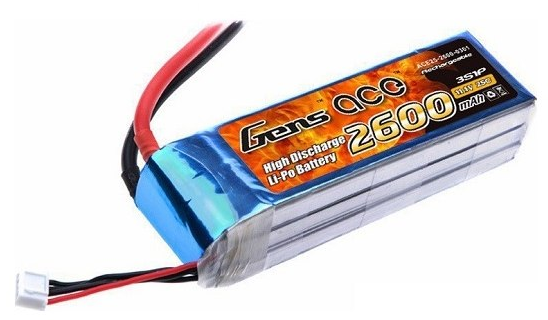
\includegraphics[scale=1]{chapter_mechanics_construction/figure2.png}
    \caption{\textit{Li-Po} аккумулятор на 2600 мА$\cdot$ч}
    \label{}
\end{figure}

С такими большими плюсами существуют и минусы, которые стоит принимать во внимание при эксплуатации такого типа аккумуляторов:
\begin{itemize}
    \item Высокая токоотдача повышает риск получить травму при работе
    \item Высоки шансы на сгорание питающейся от аккумулятора электроники в случае короткого замыкания
    \item Требуются специальные условия хранения, если аккумуляторы долгое время не используются
    \item \textit{Li-Po} аккумуляторы взрывоопасны при неправильной эксплуатации
\end{itemize}

Из-за большего опыта работы с \textit{Li-Po} аккумуляторами (несколько последних лет) и было решено использовать их. 



\section{Остальные детали}
Пластиковые детали изготовливались на \textit{3D}-принтере методом \textit{FDM} печати (послойной) из материала \textit{PET-G}. Преимущества материала для данного робота описаны ниже:
\begin{itemize}
    \item Прочность \textit{ABS}
    \item Термостойкость \textit{ABS}
    \item Долговечность \textit{ABS}
    \item Не требователен к условиям печати, как \textit{PLA}
    \item Низкая термоусадка (почти не меняет размеры при нагревании/остывании)
    \item Высокие ударопрочные свойства
    \item Возможность красить и стерилизовать
    \item Не токсичен
\end{itemize}

Может показаться что при изготовлени деталей на \textit{3D}-принтере последним можно придавать любую форму, но при \textit{FDM} технологии печати это не так. Технология достаточно дешева и может использоваться в дешевых домашних \textit{3D}-принтерах, поэтому у нее есть свои ограничения на печать <<нависающих>> над печатной областью частей детали. Поэтому при проектировании деталей из пластика нужно исходить из двух принципов. Первый заключается в том чтобы не делать новой детали из пластика, если есть альтернатива в линейке деталей, который изготавливаются по ГОСТ и продаются в специализированных магазинах. Второй принцип заключается в том чтобы использовать в детали как можно меньше материала и скомпоновать ее так, чтобы при печати максимально избежать создания поддержек для нависающих частей. Всё это накладывает свои конструктивные ограничения и требует от конструктора некоторого опыта.

\begin{figure}[h]
    \centering
    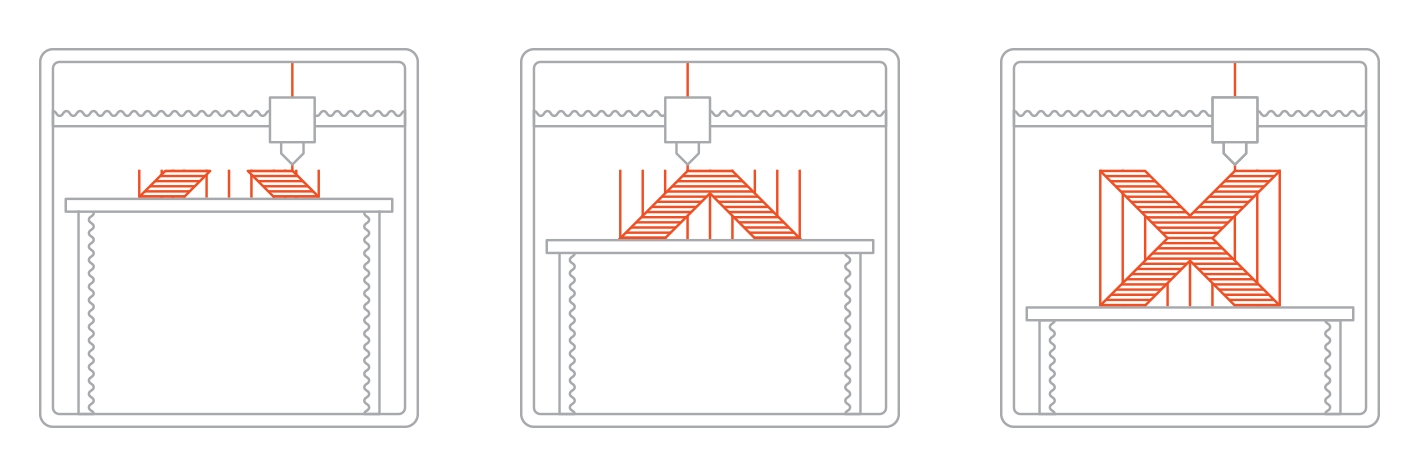
\includegraphics[scale=0.3]{chapter_mechanics_construction/figure1.png}
    \caption{Иллюстрация \textit{3D}-печати по технологии \textit{FDM}}
    \label{}
\end{figure}

Из металла выполнены покупные кронштейны, стержни ног. Стержни -- стандартные полые цилиндрические аллюминиевые профили. Подгонялись под нужную длину при помощи ножовки. Крепление к пластиковым узлам происходило вкручиванием в торцы стержней винтов. Такой способ приводит к хорошему зацеплению деталей.

Для того чтобы избежать разрушения пластиковых деталей в месте вкручивания винта в торец, и из-за невозможности нарезать резьбу в пластиковой детали, были использованы вставки из металлических гаек внутри пластикового материала.